\documentclass[11pt, oneside]{article}   
\usepackage{geometry}                	
\geometry{letterpaper}                   	
\usepackage{graphicx}		
\usepackage{amssymb}
\usepackage{applekeys}
\usepackage[T1]{fontenc}
\usepackage{menukeys}
\usepackage{enumitem}
\usepackage{chngpage}
\usepackage{multirow}
\usepackage{hyperref}
\usepackage{titlesec}

\titleclass{\subsubsubsection}{straight}[\subsection]

\newcounter{subsubsubsection}
\renewcommand\thesubsubsubsection{\thesubsubsection.\arabic{subsubsubsection}}

\titleformat{\subsubsubsection}
  {\normalfont\normalsize\bfseries}{\thesubsubsubsection}{1em}{}
\titlespacing*{\subsubsubsection}
{0pt}{3.25ex plus 1ex minus .2ex}{1.5ex plus .2ex}

\makeatletter
\def\l@subsubsubsection{\@dottedtocline{4}{7em}{4em}}
\makeatother

\setcounter{secnumdepth}{4}


\title{Dream Design of a Text Editor}
\author{Andrew Kowalczyk}
\date{December 6, 2013}						

\begin{document}
\maketitle

\section{Design}

Text editors are some of the most important pieces of software that programmers can use for their craft. I think a design of plugin for this type of an application using multiple interaction styles would be incredibly beneficial for a coder/programmer. For this particular assignment, I will model the way this plugin would work by emulating \textbf{Sublime Text 2} and \textbf{3}'s menus and actions. I will be modeling the way that voice input works by modeling it slightly after Apple OS X's Dictation utility. 

The design would mainly use audio recording from the user for all main actions. When the user simply gets tired of typing, they can revert to their spoken voice for accomplishing their goal. The ability to type in the editor is always a possibility and can be relied upon in the event of the audio recording not working as planned.

When the user would launch the application for the first time, they application would ask them to read a passage. This is like the scene in \textit{Mission: Impossible III} when Tom Cruise (disguised as Philip Seymour Hoffman) asks Philip Seymour Hoffman to read a passage \cite{mission-impossible}. This would analyze a person's accent and other vocal measurements so the application could truly understand their voice. They would then be guided through a series of tasks for them to be acquainted with the overall commands of the application. This would be comprehensive enough for them to be able to code from the get go. Also, this plugin could be modified to be an extension for any other text editor like \textit{TextWrangler}, \textit{Notepad++}, or \textit{MacVim}. This way, cross application compatibility would be accomplished. 

Certain key combinations would denote certain types of actions. Just like Dictation for Mac, pressing \keys{fn} twice would denote the start of a recording. Whenever a user will press a key or key combination once recording has started, the application would understand that the following voice input will be tailored for that action. This application would be advanced enough to be able to read and recognize variable and function names given by the user. The reason for choosing different key combinations for user input is to make the process of completing actions faster and easier for the plugin to recognize. This way the application would know what kind of input it would have to interpret.

Whenever the user begins to record, a little pox up box on the same line as the cursor would pop up and let the user know that their voice was being recorded. The purple input meter would show the loudness of the user's voice (as shown below).
\begin{center}
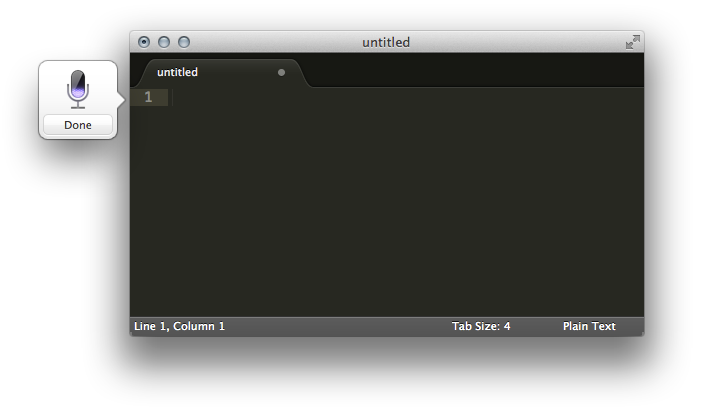
\includegraphics[width=\textwidth]{dictation.png}
\end{center}

Another option for users who have a physical disability disallowing them to hold multiple keys at a time or having a hard time moving quickly from one key to another is that the voice input could start with the commands they are trying to accomplish. For a list of all the commands, look at \ref{sec:command_table} for reference. In this document, I will be using the Mac keys for shortcuts. \keys{\cmd} denotes Command. \keys{\Alt} denotes Option or Alt. \keys{\shift} denotes Shift. \keys{\ctrl} denotes control. \keys{\Space} denotes space.

I will go through each menu bar action for Sublime Text and show how the plugin would accomplish those given actions.

\subsection{File menu \hfill \normalfont{Key: \keys{Y} Word: "file"}}


Complete a specific file menu item. Input ranges from: "save", "save as", "save all", "new file", "close file", "close all files", "open most recent", "open last closed file", "close window", and "new window". Each respective action does what it denotes.

\subsection{Edit menu \hfill \normalfont{Key: \keys{E} Word: "edit"}}

Completes a specific edit menu item. Input ranges from: "cut", "copy", "paste", "paste and indent",  "undo" and "repeat". Each respective action does what it denotes.

\subsection{Text entry, selection, manipluation, and deletion}

	\subsubsection{Entry}

		\subsubsubsection{Record \hfill \normalfont{Key: \keys{R} Word: "record"}}
		Records user input. This would allow the user to record any text they want to have entered. Keywords of whatever syntax the file is in would be recognized. Certain keywords would denote operators like +, =, |, /, etc. 

		\subsubsubsection{Record verbatim \hfill \normalfont{Key: \keys{R + V} Word: "record verbatim"}}
		Records verbatim. This would tell the application to ignore keywords and to simply record whatever input the user has provided. This would allow for saying input like "for", "equals", "pipe", etc. so that the application would not be confused with what to enter into the file.

		\subsubsubsection{Declare variables \hfill \normalfont{Key: \keys{D + V} Word: "declare variable"}}
		Declares a variable. A user's preferences and the syntax of the file that the user is working on shape the way that variables would be declared. For example, a user could define the standard to be camel casing, or underscores between words, or hyphens. This preference could be assigned by language or just generally by the user. Depending on the language variable types definitely apply.


	\subsubsection{Selection menu items \hfill \normalfont{Key: \keys{S} Word: "select"}}
	Completes a specific selection menu item. Voice input can include: "all", "word", "line", "paragraph", "scope", "indentation", and "brackets". Any of the previous commands except for "all" can be prefixed with "end of" or "beginning of" to select from the cursor to the beginning or end of the word, line, paragraph, etc. Also, input can include: "right" and "left" to move the cursor one character over in either direction.

	\subsubsection{Selection manipulation \hfill \normalfont{Key: \keys{S + M} Word: "manipulate"}}
	Manipulates a text selection. Input includes: "duplicate", "comment", "uncomment", "indent", "insert line", "next", "previous", "add next", "add previous" and "all". "indent" can be suffixed with "left" or "right". "insert line" can be suffixed with "before" and "after". If the user has selected multiple subsequent lines, another input can be "join". This joins the selection on to one line. For "next" and "previous", these would move the selection to the next or previous instance of the given selection. For "add next" and "add previous", this would add the next or previous instance of a selection to the selection. "all" would select all given instances of the given selection.


	\subsubsection{Moving text \hfill \normalfont{Key: \keys{M} Word: "move"}}
	Moves a text selection. Input that the user can provide: "up", "down", "bottom", and "top". "up" and "down" can be suffixed with any number followed by "line" or "lines". For example, "up one line" or "down seventeen lines".

	\subsubsection{Case conversion and text styles \hfill \normalfont{Key: \keys{T} Word: "style"}}
	Changes the style of a text selection. Sample input includes: "upper case" and "lower case". If a user is preparing a document using \LaTeX, some more input could be: "bold", "italic", "underlined", etc. This would allow them to change specific style of text in that document preparation system. Depending on what type of packages a user is using more commands could be defined for ease of use.

	\subsubsection{Deletion \hfill \normalfont{Key: \keys{D} Word: "delete"}}
	Delete a text selection. This works extremely similarly to text selection. All of the same inputs work in the same way except for that the simply delete the text instead of selecting it. An added input here would be "delete" for the case that the user has selected some text and then decides to delete it after the selection was made.

\subsection{Find menu items}

	\subsubsection{Find \hfill \normalfont{Key: \keys{F} Word: "find"}}
	Finds a word or phrase. Input is whatever the user wants to search for.

\subsection{Window menu and view manipulation \hfill \normalfont{Key: \keys{W} Word: "window"}}
Changes the view of the current file. Input includes: "up", "down", "page up", "page down" "top", and "bottom". "up" and "down" denote scrolling in the window. This command would also allow for an input of "minimize" to minimize a window. User inputs of "left" and "right" would cycle through the active tabs of the window in the direction that was specified.

\subsection{Tools menu items}
		
	\subsubsection{Build \hfill \normalfont{Key: \keys{B} Word: "build"}}
	Builds the file with whatever system is currently chosen. User input is: "build".

	\subsubsection{Build \hfill \normalfont{Key: \keys{B + S} Word: "build system"}}
	Changes the build system to the users input. Examples include: "Python", "Make", "C++", "\LaTeX", etc.

\subsection{Preferences \hfill \normalfont{Key: \keys{P} Word: "preferences"}}
Changes a preference. Input for this can be: "font" and  "color scheme". "font" can be suffixed with "larger" and "smaller". This command would not be able to edit preferences or package control settings due to the way \textbf{Sublime Text} stores preference files. 

\subsection{Other menu items}

	\subsubsection{File syntax \hfill \normalfont{Key: \keys{S + Y} Word: "syntax"}}
	Changes the syntax of the file. Sample input of the user includes: "Python", "C++", "\LaTeX", "Ruby on Rails", "JSON", etc.

	\subsubsection{File encoding \hfill \normalfont{Key: \keys{E} Word: "encoding"}}
	Changes the encoding of the file and reopens it. Input from the user can be: "UTF-8", "UTF-16 Little Endian", etc.

	\subsubsection{Go to line number \hfill \normalfont{Key: \keys{L} Word: "line"}}
	Moves the cursor to a certain line number. Sample input can include a specific line number or the top or bottom. Examples: "fifty-three", "first", "last", "two", etc. These inputs can prefixed with "end of" and "beginning of" to go to the end or beginning of that line. The default will be the beginning of the line. This could be changed in the user preferences.


\section{Error handling and response from the application}

In terms of being able to undo any unwanted change made by the user, the command \keys{\cmd + Z} is always available to undo a task.

In terms of error handling, if the application were to not understand what the user said, the application would prompt the user to re-speak their input after they let go of the key combination. If the input received was clearer than that, the application would do one of two things. First, if the input was extremely close to a specific keyword, variable name, etc. then it would prompt the user with, "did you mean XXX?" where XXX denotes the closest believe matching keyword, variable name, etc. If the input received was clearer yet still slightly indistinguishable between more than one keyword, the application would prompt the user a list of options that the application would believe that the user was saying. The user could then cycle through the options using "next" or "previous". If the application would prompt a user to correct something, the user would need to press \keys{\Alt + H} to respond to an error. This way the application would be able to provide positive,, specific, and constructive error messages for the user to correct their actions. In terms of providing constant feedback on the state of the application, the application would respond with "unable to complete" with a reason for not completing the action.

\section{Usage Scenarios}

	\subsection{Handicapped persons}
	The first user group that comes to mind are people who normally have some difficulty typing. Due to some physical barriers, they might be unable to input or manipulate text via the keyboard. This application would allow for the people who want to code to be able to do so. 

	\subsection{The tired coder}
	The second user group that comes to mind is the coder who is simply just tired of typing. For this target group, the technology would simply be an addition to their flow of programming. For example, when a user wants to move a piece of code into another function, this application would perform the given task faster than the typing equivalent.

\section{Rationale}

	\subsection{Mental models}
	The mental models of the designer (me) are to automate a task which is largely not automatic. Yes, there are many different applications that automatically produce code in varying ways from user input. Yet, automated code is almost always a big no-no. The mental model that this design is attempting to send across to the user is that this plugin is meant to work in conjunction with the normal commands that a user is used to using. This would not be a complete replacement of the way in which a coder could code, but more as a supplement.

	\subsection{Interaction design guidelines}
	In terms of meeting certain guidelines regarding input and data entry, this proposed design is in line with Smith and Mosier's guidelines \cite{guidelines}. They mention that a design should strive for minimal input actions by the user. By using voice, the actual amount of key presses declines sharply. The interaction with the user is simplified incredibly and allows for less doing to accomplish the same result.

	This also address the guideline that there should be a flexibility for user control of data entry. The voice input can always be used, but when a user wants to simply type out the code, they \textit{can}.

	\subsection{Interaction design principles}
	A strong principle of interaction design is to know your user, which really means that you can't know your user. The design of any application is supposed to be able to work around many different dimensions. The most important dimension that the design of this text editor addresses is the dimension of physical abilities. By making this design work for people of any physical ability (provided they can speak), it covers a large group of people. By doing so, this application can accommodate multiple user profiles. This design also contains slightly multi layered interface due to the initial help task list for the user to get acquainted with the design.

	Let's take a look and see how the design fares against some important rules of interaction design.

	First, looking at a few "golden rules" of interaction design by Shneidermann, we can see that the design proposed takes a few into consideration. It caters to universal usability and it permits easy reversal of actions \cite{shniederman-golden-rules}.

	Second, looking at Nielsen's Ten Usability Heuristics, we can see that it address some on the nose. The design proposed uses simple and natural dialog and speaks the users language. These two are the case because the user is actually using their own voice for communication. It keeps things consistent by having the shortcuts always doing the same thing. It heavily employs the use of shortcuts for ease of use. And most importantly, it address the heuristic of help and documentation by having a help sequence always available to the user \cite{nielsen-usability-heuristics}.

	Third, looking at Tognazzini's Sixteen First Principles, it also makes sure that these are addressed. It protects the users work by always allowing them to undo what they have done. The interface provided is very explorable and the user would find many new commands at their leisure to employ. It employs the first principle of human interface objects by letting the user perceive the application visually. It plays to the user other sense because voice is a large component of this interface. It has a standard way of interacting and it has standard resulting behaviors. All in all, it is understandable, self-consistent, and stable \cite{tognazzini-first-principles}.

	All in all, the interface designed approaches many rules that are seen to be very important in the way that people interact with an interface.


\section{Usability metric forecast}

	\subsection{Learnability}
	The overall learnability of the application would not be the fastest. Learning a new set of key commands is never a quick thing to lean. Also learning new phrases for certain actions for users could take a while. Since the user would be guided through a series of tasks the very first time they opened the application, this would help with the learnability. This help sequence would be available for the user to reacquaint themselves at any time with the applications commands.

	\subsection{Efficiency}
	The efficiency of the application would increase over time. As a user became more and more familiar with the flow of the application, they would be able to use the application very efficiently. Since the list of actions is fairly comprehensive, the actions that a user could accomplish via voice is nearly the same as via keyboard.

	\subsection{Errors}
	The rate of errors would decrease over time. But as imagined, they could be pretty high for a first time user. In any case, the user would be able to simply ue the keyboard to accomplish their task instead of using the voice control.

	\subsection{Memorability}
	In terms of memorability, the application would fare well. The same commands would do that same things and revisiting this application after some time would not take long to remember how the application functions. Re-familiarizing oneself with the application would be straightforward. Once again, a user could look to the series of tasks outlined in the help section to reacquaint themselves with the application.

	\subsection{Satisfaction}
	Not surprisingly, this metric is largely subjective. For people who previously had a hard time coding due to a disability, this would induce large amounts of satisfaction. For people who do not have any physical disabilities impeding them from typing, their satisfaction would rely upon how efficient they have become at using the application. The overall learning process could be slightly hard, therefore unsatisfactory.

\pagebreak
\section{Keys and words}
Here are the equivalent keys and words. \vspace{5mm}

\begin{tabular}{ | c | c | }

\hline
Key(s) & Word \\ \hline
\keys{Y} & "file" \\
\keys{E} & "edit" \\
\keys{S} & "select" \\
\keys{S + M} & "manipulate" \\
\keys{M} & "move" \\
\keys{T} & "style" \\
\keys{F} & "find" \\
\keys{R} & "record" \\
\keys{R + V} & "record verbatim" \\	
\keys{D + V} & "declare variable" \\
\keys{D} & "delete" \\
\keys{W} & "window" \\
\keys{B} & "build" \\
\keys{B + S} & "build system" \\
\keys{P} & "preferences" \\
\keys{S + Y} & "syntax" \\
\keys{E} & "encoding" \\
\keys{L} & "line" \\ \hline
\end{tabular}

\pagebreak
\newgeometry{top=1.5cm}
\section{Key command table equivalent actions}
\label{sec:command_table}
If a voice input area is blank, this means that the user can input whatever they want. If the menu action and key commands are blank, this means there is no corresponding action or commands for the voice equivalent. \vspace{5mm}

\begin{adjustbox}{center}
\begin{tabular}{ | c | c || l | l |}

\hline
Key(s) & Voice input & Menu action & Key commands\\ \hline

\multirow{10}{*}{\keys{Y}} & "save"  & \menu{File > Save} & \keys{\cmd + S}\\
	& "save as" & \menu{File > Save As..} & \keys{\shift + \cmd + S}\\
	& "save all" & \menu{File > Save All} & \keys{\Alt + \cmd + S}\\
	& "new file" & \menu{File > New File} & \keys{\cmd + N}\\ 
	& "close file" & \menu{File > Close File} & \keys{\cmd + W}\\ 
	& "close all files" & \menu{File > Close All Files} & \\ 
	& "open most recent" &  & \\ 
	& "open last closed file" & \menu{File > Open Recent > Reopen Closed File} & \keys{\shift + \cmd + T}\\ 
	& "close window" & \menu{File > Close Window} & \keys{\shift + \cmd + W}\\ 
	& "new window" & \menu{File > New Window} & \keys{\shift + \cmd + N}\\ \hline

\multirow{6}{*}{\keys{E}} & "cut" & \menu{Edit > Cut} & \keys{\cmd + X}\\
	& "copy" & \menu{Edit > Copy} & \keys{\cmd + C}\\
	& "paste" & \menu{Edit > Paste} & \keys{\cmd + V}\\
	& "paste and indent" & \menu{Edit > Paste and Indent} & \keys{\shift + \cmd + V}\\
	& "undo" & \menu{Edit > Undo} & \keys{\cmd + Z}\\
	& "repeat" & \menu{Edit > Repeat} & \keys{\cmd + Y}\\ \hline

\multirow{7}{*}{\keys{S}} & "all" & \menu{Selection > Select All} & \keys{\cmd + A}\\
	& "word" & \menu{Selection > Expand Selection to Word} & \keys{\cmd + D}\\
	& "line" & \menu{Selection > Expand Selection to Line} & \keys{\cmd + L}\\
	& "paragraph" & \menu{Selection > Expand Selection to Paragraph} & \\
	& "scope" & \menu{Selection > Expand Selection to Scope} & \keys{\shift + \cmd + \Space}\\
	& "indentation" & \menu{Selection > Expand Selection to Indentation} & \keys{\shift + \cmd + J}\\
	& "brackets" & \menu{Selection > Expand Selection to Brackets} & \keys{\ctrl + \shift + M}\\ \hline

\multirow{10}{*}{\keys{S + M}} & "duplicate" & \menu{Selection > Select All} & \keys{\cmd + A}\\
	& "comment", "uncomment"  & \menu{Edit > Comment > Toggle Comment} & \keys{\cmd + /}\\
	& "indent right" & \menu{Edit > Line > Indent} & \keys{\cmd + ]} \\
	& "indent left" & \menu{Edit > Line > Unindent} & \keys{\cmd + [} \\
	& "insert line" & \menu{Selection > Expand Selection to Scope} & \keys{\shift + \cmd + \Space}\\
	& "next" & \menu{Find > Find Next} & \keys{\cmd + G}\\
	& "previous" & \menu{Find > Find Previous} & \keys{\shift + \cmd + G}\\
	& "add next" & \menu{Find > Quick Add Next} & \keys{\cmd + D}\\
	& "add previous" &  & \\
	& "all" & \menu{Find > Quick Find All} & \keys{\ctrl + \cmd + G}\\ \hline

\multirow{4}{*}{\keys{M}} & "up" & & \\
	& "down" & & \\
	& "top" & & \\
	& "bottom" & & \\ \hline

\multirow{2}{*}{\keys{T}} & "upper case" & \menu{Edit > Convert Case > Upper Case} & \keys{\cmd + K}, \keys{\cmd + U}\\
	& "lower case"  & \menu{Edit > Convert Case > Lower Case} & \keys{\cmd + K}, \keys{\cmd + L}\\ \hline

\keys{F} & & \menu{Find > Find...} & \keys{\cmd + F}\\ \hline

\end{tabular}
\end{adjustbox}

\pagebreak

\section*{7 Key command table (cont.)}
For the command of delete, the actions that are extremely similar to text selection are deleted, the only difference is that the key commands would have \keys{Delete} after the selection commands. \vspace{5mm}

\begin{adjustbox}{center}
\begin{tabular}{ | c | c || l | l |}

\hline
Key(s) & Voice input & Menu action & Key commands\\ \hline

\multirow{2}{*}{\keys{D}} & "beginning of word" & \menu{Edit > Text > Delete Word Forward} & \\
	& "end of word" & \menu{Edit > Text > Delete Word Backward} &\\ \hline

\multirow{9}{*}{\keys{W}} & "minimize" & \menu{Window > Minimize} & \keys{\cmd + M}\\
	& "left" & \menu{Goto > Switch File > Next File} & \keys{\shift + \cmd + [}\\
	& "right" & \menu{Goto > Switch File > Previous File} & \keys{\shift + \cmd + ]}\\ 
	& "up" &  & \\ 
	& "down" &  & \\ 
	& "page up" &  & \\ 
	& "page down" &  & \\
	& "top" &  & \\
	& "bottom" &  & \\ \hline

\keys{B} & & \menu{Tools > Build} & \keys{\cmd + B} \\ \hline

\keys{B + S} & & \menu{Tools > Build System} & \\ \hline

\multirow{3}{*}{\keys{P}} & "font larger" & \menu{Sublime Text 2 > Preferences > Font > Font Larger} & \keys{\cmd + =}\\
	& "font smaller" & \menu{Sublime Text 2 > Preferences > Font > Font Smaller} & \keys{\cmd + -}\\
	& "color scheme" & \menu{Sublime Text 2 > Preferences > Color Scheme} & \\ \hline

\keys{S + Y} & & \menu{View > Syntax} & \\ \hline
\keys{E} & & \menu{File > Reopen With Encoding} & \\ \hline
\keys{L} & & \menu{Goto > Goto Line...} & \keys{\ctrl + G}\\ \hline

\end{tabular}
\end{adjustbox}

\restoregeometry

\pagebreak
\bibliography{text-editor-dream-design}
\bibliographystyle{plain}

\end{document}
	